\documentclass{article}

    % This code is generated
    \usepackage[breakable]{tcolorbox}
    \usepackage{parskip} % Stop auto-indenting (to mimic markdown behaviour)
    

    % Basic figure setup, for now with no caption control since it's done
    % automatically by Pandoc (which extracts ![](path) syntax from Markdown).
    \usepackage{graphicx}
    % Maintain compatibility with old templates. Remove in nbconvert 6.0
    \let\Oldincludegraphics\includegraphics
    % Ensure that by default, figures have no caption (until we provide a
    % proper Figure object with a Caption API and a way to capture that
    % in the conversion process - todo).
    \usepackage{caption}
    \DeclareCaptionFormat{nocaption}{}
    \captionsetup{format=nocaption,aboveskip=0pt,belowskip=0pt}

    \usepackage{float}
    \floatplacement{figure}{H} % forces figures to be placed at the correct location
    \usepackage{xcolor} % Allow colors to be defined
    \usepackage{enumerate} % Needed for markdown enumerations to work
    \usepackage[left=2cm,right=2cm, top=2cm,bottom=2cm,bindingoffset=0cm]{geometry}
    % \usepackage{geometry} % Used to adjust the document margins
    \usepackage{amsmath} % Equations
    \usepackage{amssymb} % Equations
    \usepackage{textcomp} % defines textquotesingle
    % Hack from http://tex.stackexchange.com/a/47451/13684:
    \AtBeginDocument{%
        \def\PYZsq{\textquotesingle}% Upright quotes in Pygmentized code
    }
    \usepackage{upquote} % Upright quotes for verbatim code
    \usepackage{eurosym} % defines \euro

    \usepackage{iftex}
    \ifPDFTeX
        \usepackage[T1]{fontenc}
        \IfFileExists{alphabeta.sty}{
              \usepackage{alphabeta}
          }{
              \usepackage[mathletters]{ucs}
              \usepackage[utf8x]{inputenc}
          }
    \else
        \usepackage{fontspec}
        \usepackage{unicode-math}
    \fi

    \usepackage{fancyvrb} % verbatim replacement that allows latex
    \usepackage{grffile} % extends the file name processing of package graphics
                         % to support a larger range
    \makeatletter % fix for old versions of grffile with XeLaTeX
    \@ifpackagelater{grffile}{2019/11/01}
    {
      % Do nothing on new versions
    }
    {
      \def\Gread@@xetex#1{%
        \IfFileExists{"\Gin@base".bb}%
        {\Gread@eps{\Gin@base.bb}}%
        {\Gread@@xetex@aux#1}%
      }
    }
    \makeatother
    \usepackage[Export]{adjustbox} % Used to constrain images to a maximum size
    \adjustboxset{max size={0.9\linewidth}{0.9\paperheight}}

    % The hyperref package gives us a pdf with properly built
    % internal navigation ('pdf bookmarks' for the table of contents,
    % internal cross-reference links, web links for URLs, etc.)
    \usepackage{hyperref}
    % The default LaTeX title has an obnoxious amount of whitespace. By default,
    % titling removes some of it. It also provides customization options.
    \usepackage{titling}
    \usepackage{longtable} % longtable support required by pandoc >1.10
    \usepackage{booktabs}  % table support for pandoc > 1.12.2
    \usepackage{array}     % table support for pandoc >= 2.11.3
    \usepackage{calc}      % table minipage width calculation for pandoc >= 2.11.1
    \usepackage[inline]{enumitem} % IRkernel/repr support (it uses the enumerate* environment)
    \usepackage[normalem]{ulem} % ulem is needed to support strikethroughs (\sout)
                                % normalem makes italics be italics, not underlines
    \usepackage{soul}      % strikethrough (\st) support for pandoc >= 3.0.0
    \usepackage{mathrsfs}
    

    
    % Colors for the hyperref package
    \definecolor{urlcolor}{rgb}{0,.145,.698}
    \definecolor{linkcolor}{rgb}{.71,0.21,0.01}
    \definecolor{citecolor}{rgb}{.12,.54,.11}

    % ANSI colors
    \definecolor{ansi-black}{HTML}{3E424D}
    \definecolor{ansi-black-intense}{HTML}{282C36}
    \definecolor{ansi-red}{HTML}{E75C58}
    \definecolor{ansi-red-intense}{HTML}{B22B31}
    \definecolor{ansi-green}{HTML}{00A250}
    \definecolor{ansi-green-intense}{HTML}{007427}
    \definecolor{ansi-yellow}{HTML}{DDB62B}
    \definecolor{ansi-yellow-intense}{HTML}{B27D12}
    \definecolor{ansi-blue}{HTML}{208FFB}
    \definecolor{ansi-blue-intense}{HTML}{0065CA}
    \definecolor{ansi-magenta}{HTML}{D160C4}
    \definecolor{ansi-magenta-intense}{HTML}{A03196}
    \definecolor{ansi-cyan}{HTML}{60C6C8}
    \definecolor{ansi-cyan-intense}{HTML}{258F8F}
    \definecolor{ansi-white}{HTML}{C5C1B4}
    \definecolor{ansi-white-intense}{HTML}{A1A6B2}
    \definecolor{ansi-default-inverse-fg}{HTML}{FFFFFF}
    \definecolor{ansi-default-inverse-bg}{HTML}{000000}

    % common color for the border for error outputs.
    \definecolor{outerrorbackground}{HTML}{FFDFDF}

    % commands and environments needed by pandoc snippets
    % extracted from the output of `pandoc -s`
    \providecommand{\tightlist}{%
      \setlength{\itemsep}{0pt}\setlength{\parskip}{0pt}}
    \DefineVerbatimEnvironment{Highlighting}{Verbatim}{commandchars=\\\{\}}
    % Add ',fontsize=\small' for more characters per line
    \newenvironment{Shaded}{}{}
    \newcommand{\KeywordTok}[1]{\textcolor[rgb]{0.00,0.44,0.13}{\textbf{{#1}}}}
    \newcommand{\DataTypeTok}[1]{\textcolor[rgb]{0.56,0.13,0.00}{{#1}}}
    \newcommand{\DecValTok}[1]{\textcolor[rgb]{0.25,0.63,0.44}{{#1}}}
    \newcommand{\BaseNTok}[1]{\textcolor[rgb]{0.25,0.63,0.44}{{#1}}}
    \newcommand{\FloatTok}[1]{\textcolor[rgb]{0.25,0.63,0.44}{{#1}}}
    \newcommand{\CharTok}[1]{\textcolor[rgb]{0.25,0.44,0.63}{{#1}}}
    \newcommand{\StringTok}[1]{\textcolor[rgb]{0.25,0.44,0.63}{{#1}}}
    \newcommand{\CommentTok}[1]{\textcolor[rgb]{0.38,0.63,0.69}{\textit{{#1}}}}
    \newcommand{\OtherTok}[1]{\textcolor[rgb]{0.00,0.44,0.13}{{#1}}}
    \newcommand{\AlertTok}[1]{\textcolor[rgb]{1.00,0.00,0.00}{\textbf{{#1}}}}
    \newcommand{\FunctionTok}[1]{\textcolor[rgb]{0.02,0.16,0.49}{{#1}}}
    \newcommand{\RegionMarkerTok}[1]{{#1}}
    \newcommand{\ErrorTok}[1]{\textcolor[rgb]{1.00,0.00,0.00}{\textbf{{#1}}}}
    \newcommand{\NormalTok}[1]{{#1}}

    % Additional commands for more recent versions of Pandoc
    \newcommand{\ConstantTok}[1]{\textcolor[rgb]{0.53,0.00,0.00}{{#1}}}
    \newcommand{\SpecialCharTok}[1]{\textcolor[rgb]{0.25,0.44,0.63}{{#1}}}
    \newcommand{\VerbatimStringTok}[1]{\textcolor[rgb]{0.25,0.44,0.63}{{#1}}}
    \newcommand{\SpecialStringTok}[1]{\textcolor[rgb]{0.73,0.40,0.53}{{#1}}}
    \newcommand{\ImportTok}[1]{{#1}}
    \newcommand{\DocumentationTok}[1]{\textcolor[rgb]{0.73,0.13,0.13}{\textit{{#1}}}}
    \newcommand{\AnnotationTok}[1]{\textcolor[rgb]{0.38,0.63,0.69}{\textbf{\textit{{#1}}}}}
    \newcommand{\CommentVarTok}[1]{\textcolor[rgb]{0.38,0.63,0.69}{\textbf{\textit{{#1}}}}}
    \newcommand{\VariableTok}[1]{\textcolor[rgb]{0.10,0.09,0.49}{{#1}}}
    \newcommand{\ControlFlowTok}[1]{\textcolor[rgb]{0.00,0.44,0.13}{\textbf{{#1}}}}
    \newcommand{\OperatorTok}[1]{\textcolor[rgb]{0.40,0.40,0.40}{{#1}}}
    \newcommand{\BuiltInTok}[1]{{#1}}
    \newcommand{\ExtensionTok}[1]{{#1}}
    \newcommand{\PreprocessorTok}[1]{\textcolor[rgb]{0.74,0.48,0.00}{{#1}}}
    \newcommand{\AttributeTok}[1]{\textcolor[rgb]{0.49,0.56,0.16}{{#1}}}
    \newcommand{\InformationTok}[1]{\textcolor[rgb]{0.38,0.63,0.69}{\textbf{\textit{{#1}}}}}
    \newcommand{\WarningTok}[1]{\textcolor[rgb]{0.38,0.63,0.69}{\textbf{\textit{{#1}}}}}


    % Define a nice break command that doesn't care if a line doesn't already
    % exist.
    \def\br{\hspace*{\fill} \\* }
    % Math Jax compatibility definitions
    \def\gt{>}
    \def\lt{<}
    \let\Oldtex\TeX
    \let\Oldlatex\LaTeX
    \renewcommand{\TeX}{\textrm{\Oldtex}}
    \renewcommand{\LaTeX}{\textrm{\Oldlatex}}
    % Document parameters
    % Document title
    \title{Automatic Differentiation}
    
    
    
    
    
    
    
% Pygments definitions
\makeatletter
\def\PY@reset{\let\PY@it=\relax \let\PY@bf=\relax%
    \let\PY@ul=\relax \let\PY@tc=\relax%
    \let\PY@bc=\relax \let\PY@ff=\relax}
\def\PY@tok#1{\csname PY@tok@#1\endcsname}
\def\PY@toks#1+{\ifx\relax#1\empty\else%
    \PY@tok{#1}\expandafter\PY@toks\fi}
\def\PY@do#1{\PY@bc{\PY@tc{\PY@ul{%
    \PY@it{\PY@bf{\PY@ff{#1}}}}}}}
\def\PY#1#2{\PY@reset\PY@toks#1+\relax+\PY@do{#2}}

\@namedef{PY@tok@w}{\def\PY@tc##1{\textcolor[rgb]{0.73,0.73,0.73}{##1}}}
\@namedef{PY@tok@c}{\let\PY@it=\textit\def\PY@tc##1{\textcolor[rgb]{0.24,0.48,0.48}{##1}}}
\@namedef{PY@tok@cp}{\def\PY@tc##1{\textcolor[rgb]{0.61,0.40,0.00}{##1}}}
\@namedef{PY@tok@k}{\let\PY@bf=\textbf\def\PY@tc##1{\textcolor[rgb]{0.00,0.50,0.00}{##1}}}
\@namedef{PY@tok@kp}{\def\PY@tc##1{\textcolor[rgb]{0.00,0.50,0.00}{##1}}}
\@namedef{PY@tok@kt}{\def\PY@tc##1{\textcolor[rgb]{0.69,0.00,0.25}{##1}}}
\@namedef{PY@tok@o}{\def\PY@tc##1{\textcolor[rgb]{0.40,0.40,0.40}{##1}}}
\@namedef{PY@tok@ow}{\let\PY@bf=\textbf\def\PY@tc##1{\textcolor[rgb]{0.67,0.13,1.00}{##1}}}
\@namedef{PY@tok@nb}{\def\PY@tc##1{\textcolor[rgb]{0.00,0.50,0.00}{##1}}}
\@namedef{PY@tok@nf}{\def\PY@tc##1{\textcolor[rgb]{0.00,0.00,1.00}{##1}}}
\@namedef{PY@tok@nc}{\let\PY@bf=\textbf\def\PY@tc##1{\textcolor[rgb]{0.00,0.00,1.00}{##1}}}
\@namedef{PY@tok@nn}{\let\PY@bf=\textbf\def\PY@tc##1{\textcolor[rgb]{0.00,0.00,1.00}{##1}}}
\@namedef{PY@tok@ne}{\let\PY@bf=\textbf\def\PY@tc##1{\textcolor[rgb]{0.80,0.25,0.22}{##1}}}
\@namedef{PY@tok@nv}{\def\PY@tc##1{\textcolor[rgb]{0.10,0.09,0.49}{##1}}}
\@namedef{PY@tok@no}{\def\PY@tc##1{\textcolor[rgb]{0.53,0.00,0.00}{##1}}}
\@namedef{PY@tok@nl}{\def\PY@tc##1{\textcolor[rgb]{0.46,0.46,0.00}{##1}}}
\@namedef{PY@tok@ni}{\let\PY@bf=\textbf\def\PY@tc##1{\textcolor[rgb]{0.44,0.44,0.44}{##1}}}
\@namedef{PY@tok@na}{\def\PY@tc##1{\textcolor[rgb]{0.41,0.47,0.13}{##1}}}
\@namedef{PY@tok@nt}{\let\PY@bf=\textbf\def\PY@tc##1{\textcolor[rgb]{0.00,0.50,0.00}{##1}}}
\@namedef{PY@tok@nd}{\def\PY@tc##1{\textcolor[rgb]{0.67,0.13,1.00}{##1}}}
\@namedef{PY@tok@s}{\def\PY@tc##1{\textcolor[rgb]{0.73,0.13,0.13}{##1}}}
\@namedef{PY@tok@sd}{\let\PY@it=\textit\def\PY@tc##1{\textcolor[rgb]{0.73,0.13,0.13}{##1}}}
\@namedef{PY@tok@si}{\let\PY@bf=\textbf\def\PY@tc##1{\textcolor[rgb]{0.64,0.35,0.47}{##1}}}
\@namedef{PY@tok@se}{\let\PY@bf=\textbf\def\PY@tc##1{\textcolor[rgb]{0.67,0.36,0.12}{##1}}}
\@namedef{PY@tok@sr}{\def\PY@tc##1{\textcolor[rgb]{0.64,0.35,0.47}{##1}}}
\@namedef{PY@tok@ss}{\def\PY@tc##1{\textcolor[rgb]{0.10,0.09,0.49}{##1}}}
\@namedef{PY@tok@sx}{\def\PY@tc##1{\textcolor[rgb]{0.00,0.50,0.00}{##1}}}
\@namedef{PY@tok@m}{\def\PY@tc##1{\textcolor[rgb]{0.40,0.40,0.40}{##1}}}
\@namedef{PY@tok@gh}{\let\PY@bf=\textbf\def\PY@tc##1{\textcolor[rgb]{0.00,0.00,0.50}{##1}}}
\@namedef{PY@tok@gu}{\let\PY@bf=\textbf\def\PY@tc##1{\textcolor[rgb]{0.50,0.00,0.50}{##1}}}
\@namedef{PY@tok@gd}{\def\PY@tc##1{\textcolor[rgb]{0.63,0.00,0.00}{##1}}}
\@namedef{PY@tok@gi}{\def\PY@tc##1{\textcolor[rgb]{0.00,0.52,0.00}{##1}}}
\@namedef{PY@tok@gr}{\def\PY@tc##1{\textcolor[rgb]{0.89,0.00,0.00}{##1}}}
\@namedef{PY@tok@ge}{\let\PY@it=\textit}
\@namedef{PY@tok@gs}{\let\PY@bf=\textbf}
\@namedef{PY@tok@ges}{\let\PY@bf=\textbf\let\PY@it=\textit}
\@namedef{PY@tok@gp}{\let\PY@bf=\textbf\def\PY@tc##1{\textcolor[rgb]{0.00,0.00,0.50}{##1}}}
\@namedef{PY@tok@go}{\def\PY@tc##1{\textcolor[rgb]{0.44,0.44,0.44}{##1}}}
\@namedef{PY@tok@gt}{\def\PY@tc##1{\textcolor[rgb]{0.00,0.27,0.87}{##1}}}
\@namedef{PY@tok@err}{\def\PY@bc##1{{\setlength{\fboxsep}{\string -\fboxrule}\fcolorbox[rgb]{1.00,0.00,0.00}{1,1,1}{\strut ##1}}}}
\@namedef{PY@tok@kc}{\let\PY@bf=\textbf\def\PY@tc##1{\textcolor[rgb]{0.00,0.50,0.00}{##1}}}
\@namedef{PY@tok@kd}{\let\PY@bf=\textbf\def\PY@tc##1{\textcolor[rgb]{0.00,0.50,0.00}{##1}}}
\@namedef{PY@tok@kn}{\let\PY@bf=\textbf\def\PY@tc##1{\textcolor[rgb]{0.00,0.50,0.00}{##1}}}
\@namedef{PY@tok@kr}{\let\PY@bf=\textbf\def\PY@tc##1{\textcolor[rgb]{0.00,0.50,0.00}{##1}}}
\@namedef{PY@tok@bp}{\def\PY@tc##1{\textcolor[rgb]{0.00,0.50,0.00}{##1}}}
\@namedef{PY@tok@fm}{\def\PY@tc##1{\textcolor[rgb]{0.00,0.00,1.00}{##1}}}
\@namedef{PY@tok@vc}{\def\PY@tc##1{\textcolor[rgb]{0.10,0.09,0.49}{##1}}}
\@namedef{PY@tok@vg}{\def\PY@tc##1{\textcolor[rgb]{0.10,0.09,0.49}{##1}}}
\@namedef{PY@tok@vi}{\def\PY@tc##1{\textcolor[rgb]{0.10,0.09,0.49}{##1}}}
\@namedef{PY@tok@vm}{\def\PY@tc##1{\textcolor[rgb]{0.10,0.09,0.49}{##1}}}
\@namedef{PY@tok@sa}{\def\PY@tc##1{\textcolor[rgb]{0.73,0.13,0.13}{##1}}}
\@namedef{PY@tok@sb}{\def\PY@tc##1{\textcolor[rgb]{0.73,0.13,0.13}{##1}}}
\@namedef{PY@tok@sc}{\def\PY@tc##1{\textcolor[rgb]{0.73,0.13,0.13}{##1}}}
\@namedef{PY@tok@dl}{\def\PY@tc##1{\textcolor[rgb]{0.73,0.13,0.13}{##1}}}
\@namedef{PY@tok@s2}{\def\PY@tc##1{\textcolor[rgb]{0.73,0.13,0.13}{##1}}}
\@namedef{PY@tok@sh}{\def\PY@tc##1{\textcolor[rgb]{0.73,0.13,0.13}{##1}}}
\@namedef{PY@tok@s1}{\def\PY@tc##1{\textcolor[rgb]{0.73,0.13,0.13}{##1}}}
\@namedef{PY@tok@mb}{\def\PY@tc##1{\textcolor[rgb]{0.40,0.40,0.40}{##1}}}
\@namedef{PY@tok@mf}{\def\PY@tc##1{\textcolor[rgb]{0.40,0.40,0.40}{##1}}}
\@namedef{PY@tok@mh}{\def\PY@tc##1{\textcolor[rgb]{0.40,0.40,0.40}{##1}}}
\@namedef{PY@tok@mi}{\def\PY@tc##1{\textcolor[rgb]{0.40,0.40,0.40}{##1}}}
\@namedef{PY@tok@il}{\def\PY@tc##1{\textcolor[rgb]{0.40,0.40,0.40}{##1}}}
\@namedef{PY@tok@mo}{\def\PY@tc##1{\textcolor[rgb]{0.40,0.40,0.40}{##1}}}
\@namedef{PY@tok@ch}{\let\PY@it=\textit\def\PY@tc##1{\textcolor[rgb]{0.24,0.48,0.48}{##1}}}
\@namedef{PY@tok@cm}{\let\PY@it=\textit\def\PY@tc##1{\textcolor[rgb]{0.24,0.48,0.48}{##1}}}
\@namedef{PY@tok@cpf}{\let\PY@it=\textit\def\PY@tc##1{\textcolor[rgb]{0.24,0.48,0.48}{##1}}}
\@namedef{PY@tok@c1}{\let\PY@it=\textit\def\PY@tc##1{\textcolor[rgb]{0.24,0.48,0.48}{##1}}}
\@namedef{PY@tok@cs}{\let\PY@it=\textit\def\PY@tc##1{\textcolor[rgb]{0.24,0.48,0.48}{##1}}}

\def\PYZbs{\char`\\}
\def\PYZus{\char`\_}
\def\PYZob{\char`\{}
\def\PYZcb{\char`\}}
\def\PYZca{\char`\^}
\def\PYZam{\char`\&}
\def\PYZlt{\char`\<}
\def\PYZgt{\char`\>}
\def\PYZsh{\char`\#}
\def\PYZpc{\char`\%}
\def\PYZdl{\char`\$}
\def\PYZhy{\char`\-}
\def\PYZsq{\char`\'}
\def\PYZdq{\char`\"}
\def\PYZti{\char`\~}
% for compatibility with earlier versions
\def\PYZat{@}
\def\PYZlb{[}
\def\PYZrb{]}
\makeatother


    % For linebreaks inside Verbatim environment from package fancyvrb.
    \makeatletter
        \newbox\Wrappedcontinuationbox
        \newbox\Wrappedvisiblespacebox
        \newcommand*\Wrappedvisiblespace {\textcolor{red}{\textvisiblespace}}
        \newcommand*\Wrappedcontinuationsymbol {\textcolor{red}{\llap{\tiny$\m@th\hookrightarrow$}}}
        \newcommand*\Wrappedcontinuationindent {3ex }
        \newcommand*\Wrappedafterbreak {\kern\Wrappedcontinuationindent\copy\Wrappedcontinuationbox}
        % Take advantage of the already applied Pygments mark-up to insert
        % potential linebreaks for TeX processing.
        %        {, <, #, %, $, ' and ": go to next line.
        %        _, }, ^, &, >, - and ~: stay at end of broken line.
        % Use of \textquotesingle for straight quote.
        \newcommand*\Wrappedbreaksatspecials {%
            \def\PYGZus{\discretionary{\char`\_}{\Wrappedafterbreak}{\char`\_}}%
            \def\PYGZob{\discretionary{}{\Wrappedafterbreak\char`\{}{\char`\{}}%
            \def\PYGZcb{\discretionary{\char`\}}{\Wrappedafterbreak}{\char`\}}}%
            \def\PYGZca{\discretionary{\char`\^}{\Wrappedafterbreak}{\char`\^}}%
            \def\PYGZam{\discretionary{\char`\&}{\Wrappedafterbreak}{\char`\&}}%
            \def\PYGZlt{\discretionary{}{\Wrappedafterbreak\char`\<}{\char`\<}}%
            \def\PYGZgt{\discretionary{\char`\>}{\Wrappedafterbreak}{\char`\>}}%
            \def\PYGZsh{\discretionary{}{\Wrappedafterbreak\char`\#}{\char`\#}}%
            \def\PYGZpc{\discretionary{}{\Wrappedafterbreak\char`\%}{\char`\%}}%
            \def\PYGZdl{\discretionary{}{\Wrappedafterbreak\char`\$}{\char`\$}}%
            \def\PYGZhy{\discretionary{\char`\-}{\Wrappedafterbreak}{\char`\-}}%
            \def\PYGZsq{\discretionary{}{\Wrappedafterbreak\textquotesingle}{\textquotesingle}}%
            \def\PYGZdq{\discretionary{}{\Wrappedafterbreak\char`\"}{\char`\"}}%
            \def\PYGZti{\discretionary{\char`\~}{\Wrappedafterbreak}{\char`\~}}%
        }
        % Some characters . , ; ? ! / are not pygmentized.
        % This macro makes them "active" and they will insert potential linebreaks
        \newcommand*\Wrappedbreaksatpunct {%
            \lccode`\~`\.\lowercase{\def~}{\discretionary{\hbox{\char`\.}}{\Wrappedafterbreak}{\hbox{\char`\.}}}%
            \lccode`\~`\,\lowercase{\def~}{\discretionary{\hbox{\char`\,}}{\Wrappedafterbreak}{\hbox{\char`\,}}}%
            \lccode`\~`\;\lowercase{\def~}{\discretionary{\hbox{\char`\;}}{\Wrappedafterbreak}{\hbox{\char`\;}}}%
            \lccode`\~`\:\lowercase{\def~}{\discretionary{\hbox{\char`\:}}{\Wrappedafterbreak}{\hbox{\char`\:}}}%
            \lccode`\~`\?\lowercase{\def~}{\discretionary{\hbox{\char`\?}}{\Wrappedafterbreak}{\hbox{\char`\?}}}%
            \lccode`\~`\!\lowercase{\def~}{\discretionary{\hbox{\char`\!}}{\Wrappedafterbreak}{\hbox{\char`\!}}}%
            \lccode`\~`\/\lowercase{\def~}{\discretionary{\hbox{\char`\/}}{\Wrappedafterbreak}{\hbox{\char`\/}}}%
            \catcode`\.\active
            \catcode`\,\active
            \catcode`\;\active
            \catcode`\:\active
            \catcode`\?\active
            \catcode`\!\active
            \catcode`\/\active
            \lccode`\~`\~
        }
    \makeatother

    \let\OriginalVerbatim=\Verbatim
    \makeatletter
    \renewcommand{\Verbatim}[1][1]{%
        %\parskip\z@skip
        \sbox\Wrappedcontinuationbox {\Wrappedcontinuationsymbol}%
        \sbox\Wrappedvisiblespacebox {\FV@SetupFont\Wrappedvisiblespace}%
        \def\FancyVerbFormatLine ##1{\hsize\linewidth
            \vtop{\raggedright\hyphenpenalty\z@\exhyphenpenalty\z@
                \doublehyphendemerits\z@\finalhyphendemerits\z@
                \strut ##1\strut}%
        }%
        % If the linebreak is at a space, the latter will be displayed as visible
        % space at end of first line, and a continuation symbol starts next line.
        % Stretch/shrink are however usually zero for typewriter font.
        \def\FV@Space {%
            \nobreak\hskip\z@ plus\fontdimen3\font minus\fontdimen4\font
            \discretionary{\copy\Wrappedvisiblespacebox}{\Wrappedafterbreak}
            {\kern\fontdimen2\font}%
        }%

        % Allow breaks at special characters using \PYG... macros.
        \Wrappedbreaksatspecials
        % Breaks at punctuation characters . , ; ? ! and / need catcode=\active
        \OriginalVerbatim[#1,codes*=\Wrappedbreaksatpunct]%
    }
    \makeatother

    % Exact colors from NB
    \definecolor{incolor}{HTML}{303F9F}
    \definecolor{outcolor}{HTML}{D84315}
    \definecolor{cellborder}{HTML}{CFCFCF}
    \definecolor{cellbackground}{HTML}{F7F7F7}

    % prompt
    \makeatletter
    \newcommand{\boxspacing}{\kern\kvtcb@left@rule\kern\kvtcb@boxsep}
    \makeatother
    \newcommand{\prompt}[4]{
        {\ttfamily\llap{{\color{#2}[#3]:\hspace{3pt}#4}}\vspace{-\baselineskip}}
    }
    

    
    % Prevent overflowing lines due to hard-to-break entities
    \sloppy
    % Setup hyperref package
    \hypersetup{
      breaklinks=true,  % so long urls are correctly broken across lines
      colorlinks=true,
      urlcolor=urlcolor,
      linkcolor=linkcolor,
      citecolor=citecolor,
      }
    % Slightly bigger margins than the latex defaults
    
    \geometry{verbose,tmargin=1in,bmargin=1in,lmargin=1in,rmargin=1in}
    
    



% \usepackage[utf8]{inputenc}
% \usepackage[T2A]{fontenc}
\usepackage[english,russian]{babel}
\usepackage{amsmath}
\usepackage{faktor} 
\usepackage{mathrsfs}
\usepackage{amssymb}
\usepackage{mathtools}
\usepackage{amsthm}

\DeclareMathOperator{\ord}{ord}
\DeclareMathOperator{\orb}{Orb}
\DeclareMathOperator{\stab}{Stab}
\DeclareMathOperator{\lcm}{lcm}
\DeclareMathOperator{\inn}{Inn}
\DeclareMathOperator{\Ker}{Ker}
\DeclareMathOperator{\im}{Im}
\DeclareMathOperator{\tr}{tr}
\DeclareMathOperator{\rk}{rk}
\DeclareMathOperator{\conv}{conv}

\newcommand*{\QED}{\null\nobreak\hfill\ensuremath{\square}}%
\newcommand*{\R}{\mathbb{R}}

\title{Matrix calculus}
\author{Ковалев Алексей}
\date{}

\begin{document}

\maketitle

\paragraph{1.} $f(x) = \tr(A^{\top} A x x^{\top}),\, x \in \R^n,\, A \in \R^{m \times n}$
\[ f(x) = \tr(A^{\top} A x x^{\top}) = \tr(x^{\top} A^{\top} A x) = \tr((Ax)^{\top} Ax) = (Ax)^{\top} Ax = \langle Ax,\, Ax \rangle \]
\[ df(x) =  \langle Adx,\, Ax \rangle + \langle Ax,\, Adx \rangle = \langle 2 A^{\top} A x,\, dx \rangle \]
\textbf{Ответ:} $ \nabla f(x) = 2 A^{\top} A x $


\paragraph{2.} $f(x) = \frac{1}{2} \| Ax - b \|_2^2,\, x \in \R^n,\, A \in \R^{m \times n},\, b \in \R^{m}$
\[ f(x) = \frac{1}{2} \| Ax - b \|_2^2 = \frac{1}{2} \langle Ax - b,\, Ax - b \rangle \]
\[ df(x) = \langle Ax - b,\, Adx \rangle = \langle A^{\top} (Ax - b),\, dx \rangle \]
\[ d^2 f(x) = \langle A^{\top} A dx,\, dx \rangle \]
\textbf{Ответ:} $\nabla f(x) = A^{\top} (Ax - b);\; f''(x) = A^{\top} A$


\paragraph{3.} $f(x) = \frac{1}{m} \sum\limits_{i = 1}^m \log(1 + \exp(a_i^{\top} x)) + \frac{\mu}{2} \| x \|_2^2, \, a_i, x \in \R^n, \, \mu > 0$
\[ df(x) = \frac{1}{m} \sum\limits_{i = 1}^m \frac{\exp(a_i^{\top} x) \cdot \langle a_i,\, dx \rangle}{1 + \exp(a_i^{\top} x)} + \frac{\mu}{2} \cdot 2\langle x,\, dx \rangle = \bigg\langle \frac{1}{m} \sum\limits_{i = 1}^m \frac{\exp(a_i^{\top} x)}{1 + \exp(a_i^{\top} x)} \cdot a_i + \mu x,\, dx \bigg\rangle \]
\begin{equation*}
\begin{aligned}
    d^2f(x) &= \bigg\langle \frac{1}{m} \sum\limits_{i = 1}^m \frac{\left(1 + \exp(a_i^{\top} x)\right) \cdot d\left(\exp(a_i^{\top} x)\right) - d\left(1 + \exp(a_i^{\top} x)\right) \cdot \exp(a_i^{\top} x)}{\left(1 + \exp(a_i^{\top} x)\right)^2} \cdot a_i + \mu dx,\, dx \bigg\rangle \\
    &= \bigg\langle \frac{1}{m} \sum\limits_{i = 1}^m \frac{\left(1 + \exp(a_i^{\top} x)\right) \cdot \exp(a_i^{\top} x) \cdot \langle a_i,\, dx \rangle - \exp(a_i^{\top} x) \cdot \langle a_i,\, dx \rangle \cdot \exp(a_i^{\top} x)}{\left(1 + \exp(a_i^{\top} x)\right)^2} \cdot a_i + \mu dx,\, dx \bigg\rangle \\
    &= \bigg\langle \frac{1}{m} \sum\limits_{i = 1}^m \frac{\exp(a_i^{\top} x) \cdot a_i^{\top} dx}{\left(1 + \exp(a_i^{\top} x)\right)^2} \cdot a_i + \mu dx,\, dx \bigg\rangle = \bigg\langle \bigg(\frac{1}{m} \sum\limits_{i = 1}^m \frac{\exp(a_i^{\top} x) \cdot a_i^{\top}}{\left(1 + \exp(a_i^{\top} x)\right)^2} \cdot a_i + \mu \bigg) dx,\, dx \bigg\rangle
\end{aligned}
\end{equation*}
\textbf{Ответ:} $\nabla f(x) = \frac{1}{m} \sum\limits_{i = 1}^m \frac{\exp(a_i^{\top} x)}{1 + \exp(a_i^{\top} x)} \cdot a_i + \mu x;\; f''(x) = \frac{1}{m} \sum\limits_{i = 1}^m \frac{\exp(a_i^{\top} x) \cdot a_i^{\top}}{\left(1 + \exp(a_i^{\top} x)\right)^2} \cdot a_i + \mu$


\paragraph{4.} $f(A) = \tr(e^A),\, A \in \R^{n \times n}$
\[ e^A = \sum\limits_{k = 0}^\infty \frac{1}{k!} A^k \]
\[ d(e^A) = \sum\limits_{k = 0}^\infty \frac{1}{k!} \sum\limits_{j = 0}^{k - 1} A^{j} \cdot dA \cdot A^{k - j - 1} \]
\begin{equation*}
\begin{aligned}
    df(A) &= \big\langle I,\, d(e^A) \big\rangle = \bigg\langle I,\, \sum\limits_{k = 0}^\infty \frac{1}{k!} \sum\limits_{j = 0}^{k - 1} A^{j} \cdot dA \cdot A^{k - j - 1} \bigg\rangle = \sum\limits_{k = 0}^\infty \frac{1}{k!} \sum\limits_{j = 0}^{k - 1} \big\langle I,\, A^{j} \cdot dA \cdot A^{k - j - 1} \big\rangle \\
    &= \sum\limits_{k = 0}^\infty \frac{1}{k!} \sum\limits_{j = 0}^{k - 1} \big\langle (A^j)^{\top}, dA \cdot (A^{k - j - 1})^{\top} \big\rangle = \sum\limits_{k = 0}^\infty \frac{1}{k!} \sum\limits_{j = 0}^{k - 1} \big\langle (A^j)^{\top} \cdot (A^{k - j - 1})^{\top},\, dA \big\rangle \\
    &= \sum\limits_{k = 0}^\infty \frac{1}{k!} \big\langle k (A^{k - 1})^{\top},\, dA \big\rangle = \sum\limits_{k = 0}^\infty \frac{1}{k!} \big\langle (A^{\top})^k,\, dA \big\rangle \\
    &= \big\langle \exp(A^{\top}),\, dA \big\rangle
\end{aligned}
\end{equation*}
\textbf{Ответ:} $\nabla_A f(A) = \exp(A^{\top})$


\paragraph{5.} $f(x) = \frac{1}{2} \| A - x x^{\top} \|_F^2,\, A \in \mathbb{S}^n$
\[ f(x) = \frac{1}{2} \| A - x x^{\top} \|_F^2 = \frac{1}{2} \langle A - x x^{\top},\, A - x x^{\top} \rangle \]
\begin{equation*}
\begin{aligned}
    df(x) &= \big\langle A - x x^{\top},\, d(x x^{\top}) \big\rangle = \langle A - x x^{\top},\, dx \cdot x^{\top} \rangle + \langle A - x x^{\top},\, x \cdot dx^{\top} \rangle \\
    &= \langle Ax - x x^{\top}x,\, dx \rangle + \langle x^{\top}A - x^{\top} x x^{\top},\, dx^{\top} \rangle = \langle Ax - x x^{\top}x,\, dx \rangle + \langle Ax - x x^{\top} x,\, dx \rangle \\
    &= \langle 2Ax - 2x x^{\top} x,\, dx \rangle
\end{aligned}
\end{equation*}
\begin{equation*}
\begin{aligned}
    d^2f(x) &= 2 \big\langle A dx - d(x x^{\top} x),\, dx \big\rangle = \langle 2Adx, dx \rangle - \big\langle 2dx \cdot \langle x,\, x \rangle,\, dx \big\rangle - \big\langle 2x \cdot 2 \langle x,\, dx \rangle,\, dx \big\rangle \\
    &= \big\langle (2A - 6x x^{\top})dx,\, dx \big\rangle
\end{aligned}
\end{equation*}
\textbf{Ответ:} $\nabla f(x) = 2Ax - 2xx^{\top}x;\; f''(x) = 2A - 6x x^{\top}$


\paragraph{6.} $f: S \to \R,\, f(t) = \det(A - tI),\, A \in \R^{n \times n},\, S = \{ t \in \R : \det(A - tI) \neq 0 \}$
\[ df(t) = \det(A - tI) \cdot \big\langle (A - tI)^{-\top},\, -Idt \big\rangle \]
\begin{equation*}
\begin{aligned}
    d^2f(t) &= \bigg\langle \det(A - tI) \cdot \big\langle (A - tI)^{-\top},\, Idt \big\rangle \cdot (A - tI)^{-\top},\, Idt \bigg\rangle + \det(A - tI) \cdot \big\langle (A - tI)^{-\top} \cdot Idt \cdot (A - tI)^{-\top},\, Idt \big\rangle \\
    &= \det(A - tI) \cdot \bigg\langle (A - tI)^{-\top} \cdot \Big(\big\langle (A - tI)^{-\top},\, I \big\rangle \cdot I + (A - tI)^{-\top}\Big)dt,\, Idt \bigg\rangle \\
    &= \det(A - tI) \cdot \bigg\langle (A - tI)^{-\top} \cdot \Big(\tr\left((A - tI)^{-1}\right) \cdot I + (A - tI)^{-\top}\Big)dt,\, Idt \bigg\rangle \\
    &= \det(A - tI) \cdot \Big(\tr\left((A - tI)^{-2}\right) + \tr^2\left((A - tI)^{-1}\right) \Big) dt^2
\end{aligned}
\end{equation*}
\textbf{Ответ:} $f''(t) = \det(A - tI) \cdot \Big(\tr\left((A - tI)^{-2}\right) + \tr^2\left((A - tI)^{-1}\right) \Big)$


\paragraph{7.} $f(X) = \tr\left(AX^2BX^{-\top}\right)$
\begin{equation*}
\begin{aligned}
    df(X) &= \big\langle I,\, A(dX \cdot X + X \cdot dX)BX^{-\top} - A \cdot X^2 \cdot B \cdot X^{-\top} \cdot dX^{\top} \cdot X^{-\top} \big\rangle \\
    &= \big\langle A^{\top}X^{-1}B^{\top}X^{\top},\, dX \big\rangle + \big\langle X^{\top}A^{\top}X^{-1}B^{\top},\, dX \big\rangle - \big\langle X^{-\top}AX^2BX^{-\top}, dX \big\rangle \\
    &= \big\langle A^{\top}X^{-1}B^{\top}X^{\top} + X^{\top}A^{\top}X^{-1}B^{\top} - X^{-\top}AX^2BX^{-\top},\, dX \big\rangle
\end{aligned}
\end{equation*}
\textbf{Ответ:} $\nabla f(x) = A^{\top}X^{-1}B^{\top}X^{\top} + X^{\top}A^{\top}X^{-1}B^{\top} - X^{-\top}AX^2BX^{-\top}$



\title{Automatic differentiation and jax}\label{automatic-differentiation-and-jax}
\author{}

% This code is generated

\maketitle

    \begin{tcolorbox}[breakable, size=fbox, boxrule=1pt, pad at break*=1mm,colback=cellbackground, colframe=cellborder]
\prompt{In}{incolor}{1}{\boxspacing}
\begin{Verbatim}[commandchars=\\\{\}]
\PY{k+kn}{import} \PY{n+nn}{random}

\PY{k+kn}{import} \PY{n+nn}{jax}
\PY{k+kn}{from} \PY{n+nn}{jax} \PY{k+kn}{import} \PY{n}{numpy} \PY{k}{as} \PY{n}{np}
\PY{k+kn}{from} \PY{n+nn}{jax} \PY{k+kn}{import} \PY{n}{scipy} \PY{k}{as} \PY{n}{sp}
\end{Verbatim}
\end{tcolorbox}

    \begin{tcolorbox}[breakable, size=fbox, boxrule=1pt, pad at break*=1mm,colback=cellbackground, colframe=cellborder]
\prompt{In}{incolor}{2}{\boxspacing}
\begin{Verbatim}[commandchars=\\\{\}]
\PY{k}{def} \PY{n+nf}{seed}\PY{p}{(}\PY{p}{)}\PY{p}{:}
    \PY{k}{return} \PY{n}{jax}\PY{o}{.}\PY{n}{random}\PY{o}{.}\PY{n}{PRNGKey}\PY{p}{(}\PY{n}{random}\PY{o}{.}\PY{n}{randint}\PY{p}{(}\PY{l+m+mi}{0}\PY{p}{,} \PY{l+m+mi}{228}\PY{p}{)}\PY{p}{)}
\end{Verbatim}
\end{tcolorbox}

    \begin{tcolorbox}[breakable, size=fbox, boxrule=1pt, pad at break*=1mm,colback=cellbackground, colframe=cellborder]
\prompt{In}{incolor}{3}{\boxspacing}
\begin{Verbatim}[commandchars=\\\{\}]
\PY{k}{def} \PY{n+nf}{compare\PYZus{}differentiation\PYZus{}methods}\PY{p}{(}\PY{n}{f}\PY{p}{,} \PY{n}{gradf}\PY{p}{,} \PY{n}{shape}\PY{p}{,} \PY{n}{repeat\PYZus{}times}\PY{o}{=}\PY{l+m+mi}{5}\PY{p}{)}\PY{p}{:}
    \PY{k}{for} \PY{n}{i} \PY{o+ow}{in} \PY{n+nb}{range}\PY{p}{(}\PY{n}{repeat\PYZus{}times}\PY{p}{)}\PY{p}{:}
        \PY{n}{x} \PY{o}{=} \PY{n}{jax}\PY{o}{.}\PY{n}{random}\PY{o}{.}\PY{n}{uniform}\PY{p}{(}\PY{n}{seed}\PY{p}{(}\PY{p}{)}\PY{p}{,} \PY{n}{shape}\PY{o}{=}\PY{n}{shape}\PY{p}{)}
        \PY{n}{isclose} \PY{o}{=} \PY{n}{np}\PY{o}{.}\PY{n}{isclose}\PY{p}{(}\PY{n}{gradf}\PY{p}{(}\PY{n}{x}\PY{p}{)}\PY{p}{,} \PY{n}{jax}\PY{o}{.}\PY{n}{grad}\PY{p}{(}\PY{n}{f}\PY{p}{)}\PY{p}{(}\PY{n}{x}\PY{p}{)}\PY{p}{)}\PY{o}{.}\PY{n}{flatten}\PY{p}{(}\PY{p}{)}

        \PY{n+nb}{print}\PY{p}{(}\PY{l+s+sa}{f}\PY{l+s+s2}{\PYZdq{}}\PY{l+s+s2}{Iteration }\PY{l+s+si}{\PYZob{}}\PY{n}{i}\PY{l+s+si}{\PYZcb{}}\PY{l+s+s2}{: }\PY{l+s+s2}{\PYZdq{}}\PY{p}{,} \PY{n}{end}\PY{o}{=}\PY{l+s+s1}{\PYZsq{}}\PY{l+s+s1}{\PYZsq{}}\PY{p}{)}
        \PY{k}{if} \PY{n}{np}\PY{o}{.}\PY{n}{all}\PY{p}{(}\PY{n}{isclose} \PY{o}{==} \PY{k+kc}{True}\PY{p}{)}\PY{p}{:}
            \PY{n+nb}{print}\PY{p}{(}\PY{l+s+s2}{\PYZdq{}}\PY{l+s+s2}{all components are close}\PY{l+s+s2}{\PYZdq{}}\PY{p}{)}
        \PY{k}{else}\PY{p}{:}
            \PY{n+nb}{print}\PY{p}{(}\PY{l+s+s2}{\PYZdq{}}\PY{l+s+s2}{some components differ}\PY{l+s+s2}{\PYZdq{}}\PY{p}{)}
            \PY{n+nb}{print}\PY{p}{(}\PY{l+s+sa}{f}\PY{l+s+s2}{\PYZdq{}}\PY{l+s+s2}{Max componentwise relative error is: }\PY{l+s+si}{\PYZob{}}\PY{p}{(}\PY{p}{(}\PY{n}{gradf}\PY{p}{(}\PY{n}{x}\PY{p}{)}\PY{+w}{ }\PY{o}{\PYZhy{}}\PY{+w}{ }\PY{n}{jax}\PY{o}{.}\PY{n}{grad}\PY{p}{(}\PY{n}{f}\PY{p}{)}\PY{p}{(}\PY{n}{x}\PY{p}{)}\PY{p}{)}\PY{+w}{ }\PY{o}{/}\PY{+w}{ }\PY{n}{gradf}\PY{p}{(}\PY{n}{x}\PY{p}{)}\PY{p}{)}\PY{o}{.}\PY{n}{max}\PY{p}{(}\PY{p}{)}\PY{l+s+si}{\PYZcb{}}\PY{l+s+s2}{\PYZdq{}}\PY{p}{)}
\end{Verbatim}
\end{tcolorbox}

    \hypertarget{task-1}{%
\subsection*{1.}\label{task-1}}

    \begin{tcolorbox}[breakable, size=fbox, boxrule=1pt, pad at break*=1mm,colback=cellbackground, colframe=cellborder]
\prompt{In}{incolor}{4}{\boxspacing}
\begin{Verbatim}[commandchars=\\\{\}]
\PY{k}{def} \PY{n+nf}{f}\PY{p}{(}\PY{n}{x}\PY{p}{,} \PY{n}{y}\PY{p}{)}\PY{p}{:}
    \PY{k}{return} \PY{n}{np}\PY{o}{.}\PY{n}{exp}\PY{p}{(}\PY{o}{\PYZhy{}}\PY{p}{(}\PY{n}{np}\PY{o}{.}\PY{n}{sin}\PY{p}{(}\PY{n}{x}\PY{p}{)} \PY{o}{\PYZhy{}} \PY{n}{np}\PY{o}{.}\PY{n}{cos}\PY{p}{(}\PY{n}{y}\PY{p}{)}\PY{p}{)}\PY{o}{*}\PY{o}{*}\PY{l+m+mi}{2}\PY{p}{)}
\end{Verbatim}
\end{tcolorbox}

    \begin{tcolorbox}[breakable, size=fbox, boxrule=1pt, pad at break*=1mm,colback=cellbackground, colframe=cellborder]
\prompt{In}{incolor}{5}{\boxspacing}
\begin{Verbatim}[commandchars=\\\{\}]
\PY{n}{graph} \PY{o}{=} \PY{n}{jax}\PY{o}{.}\PY{n}{xla\PYZus{}computation}\PY{p}{(}\PY{n}{f}\PY{p}{)}\PY{p}{(}\PY{n}{np}\PY{o}{.}\PY{n}{ones}\PY{p}{(}\PY{l+m+mi}{1337}\PY{p}{)}\PY{p}{,} \PY{n}{np}\PY{o}{.}\PY{n}{ones}\PY{p}{(}\PY{l+m+mi}{1337}\PY{p}{)}\PY{p}{)}
\PY{k}{with} \PY{n+nb}{open}\PY{p}{(}\PY{l+s+s2}{\PYZdq{}}\PY{l+s+s2}{graph.dot}\PY{l+s+s2}{\PYZdq{}}\PY{p}{,} \PY{l+s+s2}{\PYZdq{}}\PY{l+s+s2}{w}\PY{l+s+s2}{\PYZdq{}}\PY{p}{)} \PY{k}{as} \PY{n}{file}\PY{p}{:}
    \PY{n}{file}\PY{o}{.}\PY{n}{write}\PY{p}{(}\PY{n}{graph}\PY{o}{.}\PY{n}{as\PYZus{}hlo\PYZus{}dot\PYZus{}graph}\PY{p}{(}\PY{p}{)}\PY{p}{)}
\end{Verbatim}
\end{tcolorbox}

    \begin{Verbatim}[commandchars=\\\{\}]
WARNING: All log messages before absl::InitializeLog() is called are written to
STDERR
I0000 00:00:1695852646.751447  232267 tfrt\_cpu\_pjrt\_client.cc:349] TfrtCpuClient
created.
No GPU/TPU found, falling back to CPU. (Set TF\_CPP\_MIN\_LOG\_LEVEL=0 and rerun for
more info.)
    \end{Verbatim}

    \begin{tcolorbox}[breakable, size=fbox, boxrule=1pt, pad at break*=1mm,colback=cellbackground, colframe=cellborder]
\prompt{In}{incolor}{6}{\boxspacing}
\begin{Verbatim}[commandchars=\\\{\}]
\PY{o}{!}dot\PY{+w}{ }graph.dot\PY{+w}{ }\PYZhy{}Tpng\PY{+w}{ }\PYZgt{}\PY{+w}{ }graph.png
\end{Verbatim}
\end{tcolorbox}

\begin{figure}[H]
    \centering
    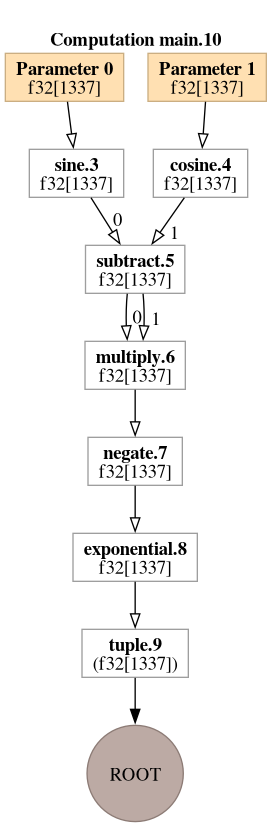
\includegraphics[scale=0.6]{graph.png}
\end{figure}

    \hypertarget{task-2}{%
\subsection*{2.}\label{task-2}}
\[ f(A) = \operatorname{tr}(e^A),\, A \in \mathbb{R}^{n \times n} \]
\[ \nabla f(A) = \exp(A^{\top}) \] proved in task 4 in Matrix calculus
hw

    \begin{tcolorbox}[breakable, size=fbox, boxrule=1pt, pad at break*=1mm,colback=cellbackground, colframe=cellborder]
\prompt{In}{incolor}{7}{\boxspacing}
\begin{Verbatim}[commandchars=\\\{\}]
\PY{k}{def} \PY{n+nf}{f}\PY{p}{(}\PY{n}{A}\PY{p}{)}\PY{p}{:}
    \PY{k}{return} \PY{n}{np}\PY{o}{.}\PY{n}{trace}\PY{p}{(}\PY{n}{sp}\PY{o}{.}\PY{n}{linalg}\PY{o}{.}\PY{n}{expm}\PY{p}{(}\PY{n}{A}\PY{p}{)}\PY{p}{)}
\end{Verbatim}
\end{tcolorbox}

    \begin{tcolorbox}[breakable, size=fbox, boxrule=1pt, pad at break*=1mm,colback=cellbackground, colframe=cellborder]
\prompt{In}{incolor}{8}{\boxspacing}
\begin{Verbatim}[commandchars=\\\{\}]
\PY{k}{def} \PY{n+nf}{gradf}\PY{p}{(}\PY{n}{A}\PY{p}{)}\PY{p}{:}
    \PY{k}{return} \PY{n}{sp}\PY{o}{.}\PY{n}{linalg}\PY{o}{.}\PY{n}{expm}\PY{p}{(}\PY{n}{A}\PY{o}{.}\PY{n}{T}\PY{p}{)}
\end{Verbatim}
\end{tcolorbox}

    \begin{tcolorbox}[breakable, size=fbox, boxrule=1pt, pad at break*=1mm,colback=cellbackground, colframe=cellborder]
\prompt{In}{incolor}{9}{\boxspacing}
\begin{Verbatim}[commandchars=\\\{\}]
\PY{n}{compare\PYZus{}differentiation\PYZus{}methods}\PY{p}{(}\PY{n}{f}\PY{p}{,} \PY{n}{gradf}\PY{p}{,} \PY{p}{(}\PY{l+m+mi}{20}\PY{p}{,} \PY{l+m+mi}{20}\PY{p}{)}\PY{p}{)}
\end{Verbatim}
\end{tcolorbox}

    \begin{Verbatim}[commandchars=\\\{\}]
Iteration 0: some components differ
Max componentwise relative error is: -3.2889554859139025e-05
Iteration 1: some components differ
Max componentwise relative error is: -3.779535472858697e-05
Iteration 2: some components differ
Max componentwise relative error is: -7.475094025721774e-05
Iteration 3: some components differ
Max componentwise relative error is: -3.283354453742504e-05
Iteration 4: some components differ
Max componentwise relative error is: -2.8257796657271683e-05
    \end{Verbatim}

    As we can see, different approaches give us different results with
maximum relative error about $10^{-5}$ or less

    \hypertarget{task-3}{%
\subsection*{3.}\label{task-3}}
\[ f(x) = \frac{1}{2} \| x \|^2,\, x \in \mathbb{R}^n \]
\[ f(x) = \frac{1}{2} \langle x,\, x \rangle \]
\[ df(x) = \langle x,\, dx \rangle \]
\[ \nabla f(x) = x \]

    \begin{tcolorbox}[breakable, size=fbox, boxrule=1pt, pad at break*=1mm,colback=cellbackground, colframe=cellborder]
\prompt{In}{incolor}{10}{\boxspacing}
\begin{Verbatim}[commandchars=\\\{\}]
\PY{k}{def} \PY{n+nf}{L}\PY{p}{(}\PY{n}{x\PYZus{}0}\PY{p}{)}\PY{p}{:}
    \PY{k}{def} \PY{n+nf}{wrapper}\PY{p}{(}\PY{n}{alpha}\PY{p}{)}\PY{p}{:}
        \PY{k}{nonlocal} \PY{n}{x\PYZus{}0}
        \PY{n}{x} \PY{o}{=} \PY{n}{x\PYZus{}0}
        \PY{k}{for} \PY{n}{i} \PY{o+ow}{in} \PY{n+nb}{range}\PY{p}{(}\PY{l+m+mi}{10}\PY{p}{)}\PY{p}{:}
            \PY{n}{x} \PY{o}{=} \PY{n}{x} \PY{o}{\PYZhy{}} \PY{n}{alpha}\PY{p}{[}\PY{n}{i}\PY{p}{]} \PY{o}{*} \PY{n}{x}
        \PY{k}{return} \PY{n}{np}\PY{o}{.}\PY{n}{linalg}\PY{o}{.}\PY{n}{norm}\PY{p}{(}\PY{n}{x}\PY{p}{)} \PY{o}{/} \PY{l+m+mi}{2}
    
    \PY{k}{return} \PY{n}{wrapper}
\end{Verbatim}
\end{tcolorbox}

    \begin{tcolorbox}[breakable, size=fbox, boxrule=1pt, pad at break*=1mm,colback=cellbackground, colframe=cellborder]
\prompt{In}{incolor}{11}{\boxspacing}
\begin{Verbatim}[commandchars=\\\{\}]
\PY{n}{x\PYZus{}0} \PY{o}{=} \PY{n+nb}{float}\PY{p}{(}\PY{n}{jax}\PY{o}{.}\PY{n}{random}\PY{o}{.}\PY{n}{uniform}\PY{p}{(}\PY{n}{seed}\PY{p}{(}\PY{p}{)}\PY{p}{,} \PY{n}{shape}\PY{o}{=}\PY{p}{(}\PY{l+m+mi}{1}\PY{p}{,}\PY{p}{)}\PY{p}{)}\PY{p}{[}\PY{l+m+mi}{0}\PY{p}{]}\PY{p}{)}
\PY{n}{alpha\PYZus{}1} \PY{o}{=} \PY{n}{jax}\PY{o}{.}\PY{n}{random}\PY{o}{.}\PY{n}{uniform}\PY{p}{(}\PY{n}{seed}\PY{p}{(}\PY{p}{)}\PY{p}{,} \PY{n}{maxval}\PY{o}{=}\PY{l+m+mf}{0.1}\PY{p}{,} \PY{n}{shape}\PY{o}{=}\PY{p}{(}\PY{l+m+mi}{10}\PY{p}{,}\PY{p}{)}\PY{p}{)}
\end{Verbatim}
\end{tcolorbox}

    \begin{tcolorbox}[breakable, size=fbox, boxrule=1pt, pad at break*=1mm,colback=cellbackground, colframe=cellborder]
\prompt{In}{incolor}{12}{\boxspacing}
\begin{Verbatim}[commandchars=\\\{\}]
\PY{n}{L}\PY{p}{(}\PY{n}{x\PYZus{}0}\PY{p}{)}\PY{p}{(}\PY{n}{alpha\PYZus{}1}\PY{p}{)}
\end{Verbatim}
\end{tcolorbox}

            \begin{tcolorbox}[breakable, size=fbox, boxrule=.5pt, pad at break*=1mm, opacityfill=0]
\prompt{Out}{outcolor}{12}{\boxspacing}
\begin{Verbatim}[commandchars=\\\{\}]
Array(0.07740642, dtype=float32)
\end{Verbatim}
\end{tcolorbox}
        
    \ldots{} :(

Gradient descent doesn't work

    \hypertarget{task-4}{%
\subsection*{4.}\label{task-4}}
\[ f(x) = -\log \det X,\, X \in \mathbb{R}^{n \times n} \]
\[ df(x) = -\frac{\det X \cdot \langle X^{-\top},\, dX \rangle}{\det X} = \langle X^{-\top},\, dX \rangle\]
\[ \nabla f(x) = -X^{-\top} \]

    \begin{tcolorbox}[breakable, size=fbox, boxrule=1pt, pad at break*=1mm,colback=cellbackground, colframe=cellborder]
\prompt{In}{incolor}{13}{\boxspacing}
\begin{Verbatim}[commandchars=\\\{\}]
\PY{k}{def} \PY{n+nf}{f}\PY{p}{(}\PY{n}{X}\PY{p}{)}\PY{p}{:}
    \PY{k}{return} \PY{o}{\PYZhy{}}\PY{n}{np}\PY{o}{.}\PY{n}{log}\PY{p}{(}\PY{n}{np}\PY{o}{.}\PY{n}{linalg}\PY{o}{.}\PY{n}{det}\PY{p}{(}\PY{n}{X}\PY{p}{)}\PY{p}{)}
\end{Verbatim}
\end{tcolorbox}

    \begin{tcolorbox}[breakable, size=fbox, boxrule=1pt, pad at break*=1mm,colback=cellbackground, colframe=cellborder]
\prompt{In}{incolor}{14}{\boxspacing}
\begin{Verbatim}[commandchars=\\\{\}]
\PY{k}{def} \PY{n+nf}{gradf}\PY{p}{(}\PY{n}{X}\PY{p}{)}\PY{p}{:}
    \PY{k}{return} \PY{o}{\PYZhy{}}\PY{n}{np}\PY{o}{.}\PY{n}{linalg}\PY{o}{.}\PY{n}{inv}\PY{p}{(}\PY{n}{X}\PY{p}{)}\PY{o}{.}\PY{n}{T}
\end{Verbatim}
\end{tcolorbox}

    \begin{tcolorbox}[breakable, size=fbox, boxrule=1pt, pad at break*=1mm,colback=cellbackground, colframe=cellborder]
\prompt{In}{incolor}{15}{\boxspacing}
\begin{Verbatim}[commandchars=\\\{\}]
\PY{n}{compare\PYZus{}differentiation\PYZus{}methods}\PY{p}{(}\PY{n}{f}\PY{p}{,} \PY{n}{gradf}\PY{p}{,} \PY{p}{(}\PY{l+m+mi}{20}\PY{p}{,} \PY{l+m+mi}{20}\PY{p}{)}\PY{p}{)}
\end{Verbatim}
\end{tcolorbox}

    \begin{Verbatim}[commandchars=\\\{\}]
Iteration 0: some components differ
Max componentwise relative error is: 1.1752022146538366e-05
Iteration 1: some components differ
Max componentwise relative error is: 1.2667936971411109e-05
Iteration 2: some components differ
Max componentwise relative error is: 0.0011747117387130857
Iteration 3: some components differ
Max componentwise relative error is: 3.3135820558527485e-05
Iteration 4: some components differ
Max componentwise relative error is: 2.0440100342966616e-05
    \end{Verbatim}

    As we can see, different approaches give us different results with
maximum relative error about $10^{-4}$ or less

    \hypertarget{task-5}{%
\subsection*{5.}\label{task-5}}
\[ f(x) = x^{\top} x x^{\top} x,\, x \in \mathbb{R}^n \]
\[ f(x) = \langle x,\, x \rangle^2 \]
\[ df(x) = 4 \cdot \langle x,\, x \rangle \cdot \langle x,\, dx \rangle = \big\langle 4 \cdot \langle x,\, x \rangle \cdot x,\, dx \big\rangle \]
\[ \nabla f(x) = 4 \cdot \langle x,\, x \rangle \cdot x \]

    \begin{tcolorbox}[breakable, size=fbox, boxrule=1pt, pad at break*=1mm,colback=cellbackground, colframe=cellborder]
\prompt{In}{incolor}{16}{\boxspacing}
\begin{Verbatim}[commandchars=\\\{\}]
\PY{k}{def} \PY{n+nf}{f}\PY{p}{(}\PY{n}{x}\PY{p}{)}\PY{p}{:}
    \PY{k}{return} \PY{p}{(}\PY{n}{x}\PY{o}{.}\PY{n}{T} \PY{o}{@} \PY{n}{x}\PY{p}{)} \PY{o}{*} \PY{p}{(}\PY{n}{x}\PY{o}{.}\PY{n}{T} \PY{o}{@} \PY{n}{x}\PY{p}{)}
\end{Verbatim}
\end{tcolorbox}

    \begin{tcolorbox}[breakable, size=fbox, boxrule=1pt, pad at break*=1mm,colback=cellbackground, colframe=cellborder]
\prompt{In}{incolor}{17}{\boxspacing}
\begin{Verbatim}[commandchars=\\\{\}]
\PY{k}{def} \PY{n+nf}{gradf}\PY{p}{(}\PY{n}{x}\PY{p}{)}\PY{p}{:}
    \PY{k}{return} \PY{l+m+mi}{4} \PY{o}{*} \PY{p}{(}\PY{n}{x}\PY{o}{.}\PY{n}{T} \PY{o}{@} \PY{n}{x}\PY{p}{)} \PY{o}{*} \PY{n}{x}
\end{Verbatim}
\end{tcolorbox}

    \begin{tcolorbox}[breakable, size=fbox, boxrule=1pt, pad at break*=1mm,colback=cellbackground, colframe=cellborder]
\prompt{In}{incolor}{18}{\boxspacing}
\begin{Verbatim}[commandchars=\\\{\}]
\PY{n}{compare\PYZus{}differentiation\PYZus{}methods}\PY{p}{(}\PY{n}{f}\PY{p}{,} \PY{n}{gradf}\PY{p}{,} \PY{p}{(}\PY{l+m+mi}{100}\PY{p}{,}\PY{p}{)}\PY{p}{)}
\end{Verbatim}
\end{tcolorbox}

    \begin{Verbatim}[commandchars=\\\{\}]
Iteration 0: all components are close
Iteration 1: all components are close
Iteration 2: all components are close
Iteration 3: all components are close
Iteration 4: all components are close
    \end{Verbatim}


\end{document}
